\documentclass[12pt,preprint]{aastex}
\usepackage{url}
\usepackage{natbib}
\usepackage{graphicx}
%\usepackage{subfig}
%\usepackage{fixltx2e}

%%%%%%%%%%%%%%%%%%%%%%%%%%%%%%%%%%%%%%%%%%%%%%%%%%%%
%%% author-defined commands
\newcommand\x         {\hbox{$\times$}}
\def\mic              {\hbox{$\mu{\rm m}$}}
\def\about            {\hbox{$\sim$}}
\def\Mo               {\hbox{$M_{\odot}$}}
\def\Lo               {\hbox{$L_{\odot}$}}

%\captionsetup[figure]{labelformat=simple}
%%%%%%%%%%%%%%%%%%%%%%%%%%%%%%%%%%%%%%%%%%%%%%%%%%%%

% Abstract

% Role of MOPS
% - Inputs and Responsibilities of MOPS : generating the Moving Objects table
% - Uses of Moving Objects table: Association and Science Users

% MOPS Functionality
% - SW standards/implementation status
% - Overview of history/refs (PS-MOPS, IOD)

% MOPS Sky-Plane Tracking:
% - Overview of system (tracklets, tracks, sky-plane tracking)
% - FindTracklets and algorithms
% - Tracklet Optimizations (collapseTracklets, subset removal) 
% - Metrics and graphs of SSM distributions in velocity
% - LinkTracklets (Kubica Algorithm) 
% - Track Filters (chi-squared, subset removal)
% - Metrics and graphs of SSM distributions in acceleration + velocity
% - IOD references



\begin{document}

\title{Moving Object Pipeline Requirements}

\author{}

\begin{abstract}

The Moving Object Pipeline System (MOPS) has two responsibilities
within LSST Data Management.  First, it is responsible for generating
and managing the \textbf{Moving Object} data products.  The Moving
Objects are identified solar system objects (SSOs) with associated
Keplerian orbits, errors, and a detected sources assocated with those
solar system objects.  The second responsibility of the MOPS is to
predict future locations of moving objects in incoming images so that
their sources may be associated with known objects; this will reduce
the number of transient detections and prevent Alert Generation on
detections of known Solar System objects.

\end{abstract}

\tableofcontents

%\section{Science Requirements}

\section{System Design and Responsibilities}

The Moving Object Pipeline System has two main responsibilities: the
generation and maintenance of the Moving Object database, and the
prediction of known object locations which are sent to the Association
Pipeline to prevent unneccessary alerts.  In order to fulfill these
goals, the MOPS has been broken into several componenets, colloquially
known as ``DayMOPS'' and ``NightMOPS.''
 

\begin{figure}[!ht]
\begin{center}
  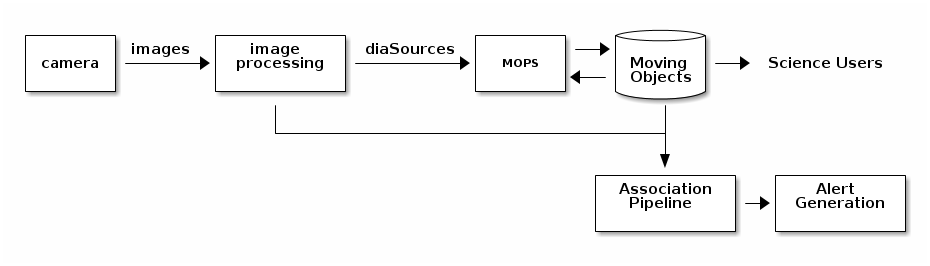
\includegraphics[width=13cm]{illustrations/mopsWithinLsst.png}
\end{center}
\caption{ Data flow from the camera through DayMOPS to the Science
  Users and Alert Generation.  DayMOPS will build and maintain the
  Moving Objects table, NightMOPS will use the Moving Objects table to
  communicate with the Assocation Pipeline.  }
\label{mopsWithinLsst}
\end{figure}


``DayMOPS,'' so called because it processes data acquired from the
previous night in a large batch operation, is responsible for
discovering new Moving Objects in newly-acquired data, searching old
data for detections of new objects, and updating the Moving Objects
table to reflect newly-acquired data. It is also responsible for
periodically cleaning and refining the contents of the Moving Objects
table.

``NightMOPS'' is responsible for projecting the locations of known
Moving Objects in upcoming images as they are announced during
night-time operations.  If Moving Objects are observed in these
images, then the Moving Object table is modified to add these
newly-acquired detections to their associated Moving Object.

The relationship between DayMOPS, NightMOPS and the neighboring
components of the LSST Data Management system is illustrated in
figure \ref{mopsWithinLsst}.

\subsection{DayMOPS: Discovering and Managing Moving Objects}

% Illustration of DayMOPS

% sky-plane vs. orbit-space illustration

The initial task of DayMOPS is to identify unknown objects present in
images and their orbits.  To accomplish this, the system initially
finds sets of detections which follow a sky-plane path roughly
consistent with asteroid motion; these sets of detections and their
fitted paths are called \textbf{tracks}.  This same method is the
basis for asteroid discovery used in the PanSTARRS Moving Object
Pipeline System \citep{psMOPSDesign}.  A set of algorithms for the
discovery of sky-plane tracks in dense data are presented in
\citet{Kubica:2005:MTA:1081870.1081889}; these algorithms are used in
the PanSTARRS MOPS as well.  Because of the loose approximations used,
many of the tracks will be mislinkages, combining detections which are
not attributable to the same source, but virtually all objects for
which a true (correctly-linked) track could be generated will get some
correct track.  LSST Data Management has developed additional
processing phases and filters which can improve the performance of the
system and reduce the computational costs by managing the number of
untrue or redundant tracks throughout the various phases of
processing.

Once tracks are discovered, they are sent to the Orbit Determination
phase. The Orbit Determination phase takes these sets of sky-plane
detections and attempts to find a Kepler orbit which could generate
the detections, if any exists.  This orbit is further refined, and
error bounds are established, using least-squares linearization.
Orbit Determination will reject many tracks as false, but should
successfully find fairly precise orbits for virtually all correctly
linked tracks.  Several methods for performing this task are known,
and several have implementations available to LSST
\citep{Milani04orbitdetermination}, \citep{Milani2006},
\citep{OpenOrb2009}, \citep{granvik_thesis}.  These orbits, and the
detections present in the track associated with that orbit, are used
to generate new Moving Objects.

\begin{figure}[h]
\begin{center}
  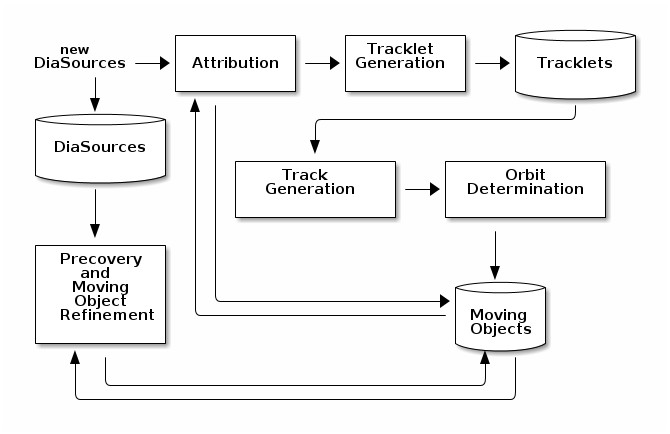
\includegraphics[width=11cm]{illustrations/mopsDiagram.png}
\end{center}
\caption{ Data flows into the DayMOPS pipeline and results in
  modifications of the Moving Objects table in a variety of ways,
  including attribution to known objects, a multi-stage pipeline for
  the discovery of new objects, and periodic refinements of the Moving
  Object table, such as possible merges of redundant objects or
  removal of false orbits. }
\label{mopsDiagram}
\end{figure}



As in the PanSTARRS MOPS design \citep{psMOPSDesign} the LSST's
DayMOPS is expected to perform several additional tasks to manage and
improve the Moving Objects table over time.  Attribution is the
process of identifying known objects in incoming data and adding those
detections to the correct Moving Object (this task is delegated to
NightMOPS). Similarly, Precovery is the recovery of known,
unattributed detections associated with a newly-discovered Moving
Object.  Another refinement is the merging of potentially redundant
Moving Objects.  The complete set of DayMOPS tasks and their data
flows are illustrated in figure \ref{mopsDiagram}.



\subsubsection{Building Tracklets}

% possible illustration: show Dec/time for two images, then tracklets in Dec/time

\textbf{Tracklets} are the building blocks of the sky-plane
\textbf{tracks} used by DayMOPS.  Tracklets are linkages between
DiaSource detections occuring within the same night; during this time
period, solar system object motion is linear or near-linear on the
sky. By creating tracklets, DayMOPS can find sky-plane position and
velocity estimates for sets of detections which may belong to solar
system objects.  This filters out many detections of non-solar system
objects, as they are less likely to generate tracklets.  The use of
tracklets also simplifies the downstream work of track generation,
which attempts to find sets of detections with a good
position/velocity/acceleration fit on the sky-plane; since tracklets
have known position and velocity, the track generation phase needs
only to find those tracklets compatible within some acceleration
factor.

In order to ensure that tracklet-generating images are acquired, it is
necessary to ensure that regions of the sky is visited two or more
times within an accepted time period within a night.  Currently, we
require that sky fields be revisited within a fairly short time period
($\leq 90$ minutes is the current rule) in order to constrain the
maximum apparent motion of solar system objects and thus also
constrain the number of tracklets.

The discovery of tracklets can be accomplished efficiently using
KD-Tree structures \citep{bentley_kdtrees} and methods from
\citet{kubica_thesis}.  DayMOPS will build a 2-dimensional (RA, Dec)
KD-Tree for each image, using the tree to hold the detections found in
that image.  Because KD-Trees allow quick range searches of
arbitrary-dimensional spatial data, it is possible to efficiently
perform searches over the detections to find pairs of detections
sufficiently close within time and within limits on apparent
velocity. These pairs of detections are linked to generate tracklets.
% TBD: Is this clear?!

% psuedo code?

Further refinements of tracklets are possible with additional
processing. If an object gets more than one tracklet, it is possible
to use methods similar to the Hough transform (CITE HOUGH, SELF) to
identify and merge these redundant tracklets into larger tracklets,
improving the linear position/velocity fits of the tracklets and
reducing the number of tracklets passed downstream.

\subsubsection{Building Tracks}

Over the course of roughly one month, solar system objects tend to
follow a roughly quadratic path on the sky-plane
\citep{kubica_thesis}.  The track generation phase of DayMOPS will
attempt to find sets of tracklets (which have position and velocity
estimates) which were observed within one month of each other and are
compatible within some sky-plane acceleration factor.  Tracks which
are suitable for generating a reasonable orbital fit are sent to the
Orbit Determination phase. 

The methods used for tracklet-to-tracklet linking are described in
\citet{kubica_thesis} and \citet{Kubica:2005:MTA:1081870.1081889}.
The methods described attempt to efficiently find sets of tracklets
which are \textit{compatible} in the sense that they could be joined
to form a track: that is, tracklets which span multiple nights and
have positions and velocities which are consistent with a fixed
acceleration.  

To perform this work efficiently, these methods use four-dimensional
KD-Trees over \textit{tracklets-space}, or (RA position, Dec position,
RA velocity, Dec velocity). One tree is created per image, and holds
each tracklet which has its first detection in that image.  A
multi-tree walk is performed using a clever algorithm, efficiently
discovering all regions of tracklet-space which could contain sets of
tracklets that are compatible, while avoiding visits to tracklet-space
regions which are not compatible and could not generate a track.  This
is performed recursively until leaf nodes of the KD-Trees are reached.

% illustration from Kubica?

When the algorithm encounters a set of leaf nodes in the KD-Trees, it
attempts to build a track using the detections held in the tracklets
at the leaf nodes.  A quadratic fit, or a higher-order fit if
possible, to the detections will be attempted.  Then a quality-of-fit
assessment is used to determine whether the track is considered
acceptably credible to pass downstream to the Orbit Determination.
Investigation into ideal quality-of-fit metrics is ongoing, but as of
this writing a filter on minimum chi-squared probability appears to be
the best option.



\subsection{NightMOPS: Predicting Moving Object Locations}

The NightMOPS section of MOPS is responsible for predicting the
locations of known Moving Objects as images are taken, so that they
may be attributed to the known Moving Objects and removed from the set
of unknown transients detections.  This allows attribution for known
Moving Objects, improving the quality of the Moving Object data
products, and also allows the prevention of unnecessary Alerts.

Predicting the locations of objects given an orbit can be accomplished
through ephemeris calculation using existing orbit-space software
suites \citep{Milani2006}, \citep{OpenOrb2009}.  However, ephemeris
calculation can be fairly slow due for large data sets.  Because the
observations schedule for LSST will be determined dynamically, it is
necessary to generate ephemeris predictions for a large Moving Object
table in a short period of time.

% some kind of time-domain illustration?

In order to accomplish this, NightMOPS will generate ``coarse
ephemerides'' for known objects, predicting their locations at the
beginning and end of the night.  Then, when given an upcoming image
location, NightMOPS will use interpolation of the coarse ephemerides
to find objects which could feasibly be present in the upcoming
image. Precise ephemerides for just these objects will be
generated. In this way, NightMOPS will avoid the problem of generating
ephemeris for each known Moving Object for every image time.


\subsection{Implementation Status}

All software components of MOPS, with the possible exception of
initial orbit determination, and orbital least-squares linearization
fitting of orbits to data, and ephemeris generation, is expected to be
completed in open-source C++ compliant with LSST software guidelines
and in LSST appropriate coding style.  These components will run
inside the LSST Pipeline Framework.  

Currently, the initial tracking phases of DayMOPS are implemented in
LSST-compliant C++.  The selection of an appropriate package for
initial orbit determination, least-squares linearization of orbit
fitting, and ephemeris generation is incomplete but several FORTRAN
options are available to us, some open-source.  A Python-based
implementation of NightMOPS, using the LSST Pipeline Framework, is
complete but it is currently using a closed-source ephemeris
generation tool.




\section{MOPS Metrics \& Scaling}

Current development efforts have focused on the sky-plane tracking
phase of DayMOPS, as all later processing hinges on its
success. Existing orbit determination packages claim a high rate of
success for accurate initial orbit determination (IOD) given a
correctly linked track, and a low rate of false positives
\textbf{(TBD: CITE)}. As a result, we expect that the ability of the
system to successfully generate Moving Objects data products for solar
system objects given to DayMOPS will be determined primarily by the
sky-plane tracking component and its ability to send useful tracks to
IOD.  We also expect the overall resource usage of the DayMOPS system
will be calculable given the runtime of the sky-plane tracking
component, the number of tracks it passes to IOD, and the per-track
IOD time of our IOD package.  As a result, carefully studying the
behavior and output of the sky-plane linking should provide a
reasonable estimate of the resource usage of all of DayMOPS.

% NightMOPS RESOURCE USAGE?!

In this section, we will present metrics used to evaluate the
usefulness of the sky-plane tracking approach, the correctness of our
software implementation, and usefulness of filters. We also
investigate the total cost of running our software and expected cost
of performing IOD on its output.


\subsection{Limits on Findability of Solar System Objects}

The requirements of IOD and practical limitations of the sky-plane
linking approach both limit the feasibility of deriving a Moving
Object for a given solar system object.  As an extreme example,
consider the case of an object observed exactly once during the survey
- it is clearly impossible to generate an orbit which precisely
predicts the motion of such an object.

Objects which are observed such that their detections meet the
requirements for IOD and sky-plane linking are considered ``findable''
objects and we reasonably expect DayMOPS to generate Moving Objects
for them.  Objects which do \textit{not} meet these requirements are
considered ``unfindable'' objects.  It is the responsibility of the
telescope Operations to ensure that a large number of objects are
observed such that they are ``findable'' for MOPS.  The current
implementation of simulated telescope operations take into account
these requirements when generating simulated sets of telescope
pointings. \textbf{reference to another chapter in the full document?}

Currently, we define an object as ``findable'' if, on three or more
nights within a span of thirty days, it generates three
tracklets. These tracklets must be made of two or more detections
which occur within a user-specified time interval.  Further, these
tracklets must have an apparent velocity below the user-specified
limit. Further, the best-fit quadratic fit of the detections in these
tracklets must have an apparent acceleration which is also below a
user-specified limit.

IOD should be capable of fitting an accurate orbit to any
correctly-linked track which fulfills the above criteria
\textbf{(CITE: Milani? Chesley?)} because they are guaranteed to have
at least six detections on three distinct nights.  


\subsubsection{Establishing Time, Velocity and Acceleration Limits}

Setting limits on tracklet velocity, track acceleration and time
intervals for the generation of tracks and tracklets is necessary for
practical reasons.  Setting overzealously low limits will reduce the
number of objects which can be found; however, as these limits are
relaxed, the number of potential mislinkages can grow quickly, greatly
increasing the computational workload.  By carefully choosing the
limits used in sky-plane linking, one can significantly reduce the
resource usage of the total DayMOPS pipeline while still extracting
useful tracks.  In this section, we will discuss the reasons for
setting these limits, present some of the limits we have chosen for
experiments, and justify those choices.

\paragraph{Velocity and Time Interval Limits For Tracklet Generation}

The first stage of the DayMOPS pipeline is tracklet generation, in
which the software identifies pairs of detections which could be
attributable to the same object.  To limit the number of incorrectly
linked tracklets, it is necessary to establish limits on the maximum
apparent velocity of tracklets as well as the maximum time interval
between two detections for tracklet generation to be attempted.  Given
a query detection, the velocity and time limit together establish the
size of the sky-plane space searched for possible paired detections,
and thus constrain the number of possible linkages.

A casual study in \citet{kubica_thesis} and experiences related to us
from work on the PanSTARRS MOPS both state an upper time limit of 90
minutes is necessary to prevent excessively high numbers of
mislinkages. A 15-minute lower limit was also suggested as a minimum
for most objects to generate useful apparent motion relative to
astrometric errors. These figures were accepted by the LSST and used
in the cadence design and cadence simulations generated with the
Operations Simulator.  

Reasonable upper limits on tracklet max velocity can be reached with a
survey of apparent motion of objects.  We carried out a survey of
apparent motion of objects in the realistic Solar System Model
presented in \citet{Grav2011}.

\textbf{VELOCITY HISTOGRAM HERE, WITH EXPLANATORY TEXT}

After study, we decided that an upper limit of .5 deg/day would be
sufficient for all objects except Near-Earth Objects
(NEOs). \textbf{Exact numbers?}




\paragraph{Acceleration and Time Interval Limits for Track Generation}

Colloquial knowledge provided by PanSTARRS claims that the quadratic
approximation of asteroid motion tends to break down when a track
spans more than 30 days of observation.  Since the quadratic
assumption is critical to sky-plane tracking, it is necessary to
impose an additional limit on the maximum time span for tracks. 

As a result, our software can examine data spanning at most 30 days
when searching for tracks.  One can imagine the software as passing a
sliding window over the data, looking for tracks which can be found
within the windowed data.  This leads us to define a \textbf{tracking
  window length}, describing the size of the window.  Objects for
which no track can be generated within this time window are also
considered ``unfindable,'' since limitations of sky-plane tracking
prevent us from building a track for them.  In order to speed up
testing of the system, we sometimes use shorter tracking windows,
which reduce the number of potentially findable objects in the data
but allow faster operation.

Further, the generation of quadratic tracks from the linear tracklets
requires an upper bound on track acceleration.  As with establishing a
velocity limit, it is possible to perform a study of objects to choose
a reasonable upper limit on track acceleration.  Again, the Solar
System Model from \citet{Grav2011} was used to generate a histogram of
apparent accelerations of objects, and this was used to establish a
reasonable upper bound on track acceleration.

\textbf{ACCELERATION HISTOGRAM HERE, WITH EXPLANATORY TEXT}

We concluded from our survey that an upper bound .02 deg/day$^2$ was
sufficient to find virtually all objects.



\subsection{Predicting Resource Usage of the System}
cut?
\subsection{Track and Tracklet Quality Metrics}
cut?
\subsection{Main-Belt Searching On Ecliptic}
results go here
\subsection{Scaling On Solar System Model Density}
results go here
\subsection{Scaling On Non-Solar System Detection Density}
results go here
\subsection{NightMOPS Resource Usage}


















\section{Development Plan}

Though the core algorithms of MOPS have been implemented in
LSST-appropriate style, further research and development are needed.

\subsection{Increasing The Number of Findable Objects}

\subsection{Exploring NEO Capability}

\subsection{Distribution/Parallelization of Core Algorithms}





\bibliographystyle{apj}
\bibliography{baseline}

\end{document}
